\documentclass{article}

\usepackage[T2A]{fontenc}
\usepackage[utf8]{inputenc}
\usepackage[russian]{babel}
\usepackage[margin=2cm]{geometry}
\usepackage{graphicx}
\usepackage{fancyvrb}
\usepackage{url}


\begin{document}
    \begin{flushright}
        \textit{Выполнил: Максимов Н. Д.} \\
        \textit{Группа: 09-414} \\
        \textit{Вариант: 8}
    \end{flushright}

    \begin{center}
        \bfseries\LARGE Отчет по лабораторной работе №1
    \end{center}
    \bigskip

    \section{Характеристики выборки}
    Исследуемая выборка имеет следующие статистические xарактеристики:
    \begin{enumerate}
        \item Объем выборки: 89
        \item Минимум: 115.0
        \item Максимум: 126.0
        \item Размах: 11.0
        \item Математическое ожидание: 121.02
        \item Выборочная дисперсия: 5.05
        \item Выборочная дисперсия (несмещенная): 5.1
        \item Стандартное отклонение: 2.25
        \item Коэффициент ассиметрии: $-0.15$
        \item Медиана: 121.2
        \item Интерквартильная широта: 3.5
    \end{enumerate}

    \section{Гистограмма и ЭФР}
    По полученной гистограмме можно сделать вывод, что мода исследуемой выборки находится в диапозоне от 112.07 до 123.64. Отрицательный коэффициент асимметрии, полученный в выше, полностью подтверждается формой гистограммы: её пик (мода) смещен вправо.
    \begin{figure}[htbp]
        \centering
        \begin{minipage}{0.5\textwidth}
            \centering
            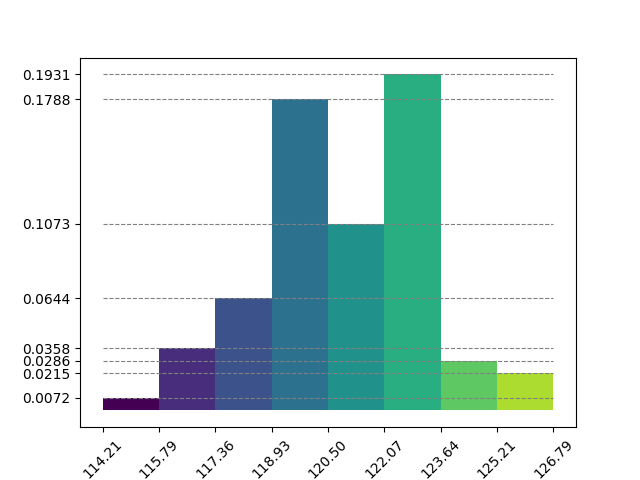
\includegraphics[width=\textwidth]{гистограмма.png}
            \caption{Гистограмма}
        \end{minipage}
        \hspace{-10pt}
        \begin{minipage}{0.5\textwidth}
            \centering
            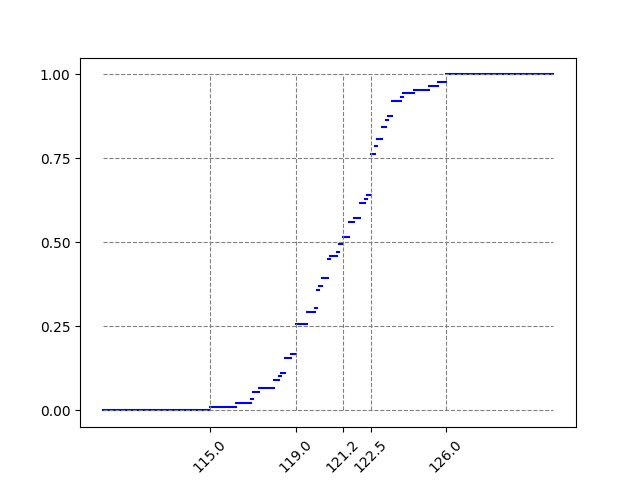
\includegraphics[width=\textwidth]{эфр.png}
            \caption{ЭФР}
        \end{minipage}
    \end{figure}

    \section{Листинг}
    \noindent \texttt{statools.py}
    \VerbatimInput[tabsize=4, fontsize=\small, numbers=left]{../source/statools.py}
    \noindent \texttt{plotools.py}
    \VerbatimInput[tabsize=4, fontsize=\small, numbers=left]{../source/plotools.py}
    \noindent \texttt{main.py}
    \VerbatimInput[tabsize=4, fontsize=\small, numbers=left]{../source/main.py}

    \bigskip
    \noindent\rule{\textwidth}{0.4pt}
    \small Полный исходный код лабораторной работы доступен в репозитории на GitHub: \url{https://github.com/mndkpfu/MS}
\end{document}